\documentclass[slidestop,compress,red,mathserif]{beamer}

\usepackage{pgf,pgfarrows,pgfnodes,pgfautomata,pgfheaps,pgfshade}
\usepackage{amsmath,amssymb}
\usepackage{comment}
\usepackage{graphicx}
\usepackage[english]{babel}
\usepackage{tabularx}
\usepackage{xcolor}
\usepackage{multirow}
\usepackage{marvosym}
\usepackage{natbib}
\usepackage{ulem}
\usepackage{wasysym}
\usepackage{setspace}

\setbeamersize{text margin left=6mm, text margin right=2mm}

\mode<presentation>
{
%\usetheme{Warsaw}
%\usetheme{Rochester}
%\usetheme{Madrid}
%\usetheme{Pittsburgh}
%\usetheme{Antibes}
%\usetheme{Montpellier}
%\usetheme{Berkeley}
%\usetheme{PaloAlto}
%\usetheme{Goettingen}
%\usetheme{Marburg}
%\usetheme{Hannover}
%\usetheme{Berlin}
\usetheme{Ilmenau}
%\usetheme{Dresden}
%\usetheme{Darmstadt}
%\usetheme{Frankfurt}
%\usetheme{Singapore}
%\usetheme{Szeged}
%\usetheme{Copenhagen}
%\usetheme{Malmoe}
\setbeamercovered{transparent}
}

% Choose color scheme
%
%\usecolortheme{default}
%\usecolortheme{sidebartab}
%\usecolortheme{albatross}
%\usecolortheme{beetle}
%\usecolortheme{crane}
%\usecolortheme{dove}
%\usecolortheme{fly}
%\usecolortheme{seagull}
%\usecolortheme{lily}
\usecolortheme{orchid}

\beamertemplateballitem
%\setbeamertemplate{footline}{\insertframenumber/\inserttotalframenumber}

\defbeamertemplate*{footline}{shadow theme}
{%
  \leavevmode%
  \hbox{\begin{beamercolorbox}[wd=2.\paperwidth,ht=2.5ex,dp=1.125ex,leftskip=.3cm plus1fil,rightskip=.3cm]{author in head/foot}%
    \usebeamerfont{author in head/foot}\insertframenumber\,/\,\inserttotalframenumber\hfill%\insertshortauthor
  \end{beamercolorbox}%
  \begin{beamercolorbox}[wd=.5\paperwidth,ht=2.5ex,dp=1.125ex,leftskip=.3cm,rightskip=.3cm plus1fil]{title in head/foot}%
    \usebeamerfont{title in head/foot}%\insertshorttitle%
  \end{beamercolorbox}}%
  \vskip0pt%
}

% number sets
\def\N{\hbox{I \kern-.5em N}}
\def\R{\hbox{I \kern-.5em R}}
\def\Q{\hbox{\hspace*{.25em}{\sf I} \kern-.83em Q}}
\def\T{\rm T}  %%%%  \rm pour roman (ecriture normale)
\def\Z{\rm Z}
\def\ZZ{\hbox{\sf  Z \kern-.8em Z}}
\def \Zplus        {\ZZ^{+}}
\def \bigm {\textsc{penal}}
\def \dst {\textsc{dst}}
\def \src {\textsc{src}}
\def \zlp {z^{\star}_{\textsc{lp}}}
\def \zilp {{\tilde z}_{\textsc{ilp}}}
\def \l    {\textnormal{\textsc{l}}}
\def \Gp   {G_{\textsc{p}}}
\def \Gl   {G_{\l}}
\def \Vp   {V_{\textsc{p}}}
\def \Vl   {V_{\l}}
\def \Ep   {E_{\textsc{p}}}
\def \El   {E_{\l}}
\def \cost {\textsc{cost}}
\def \srlg {\textsc{srlg}}

% number sets
\def \best {\textsc{best}}
\def  \N            {\hbox{I \kern-.5em N}}
\def \RR {\mathbb{R}}
\def \Rplus {\RR^+}
\def  \Z            {\rm Z}
\def  \Zplus        {\Z^+}
\def  \Zplusn       {\Zplus_n}
\def  \ZZ           {\hbox{\sf  Z \kern-.8em Z}}
\def \Z {\mathbb{Z}}

\logo{%
    
\includegraphics[width=2.cm,keepaspectratio]{Figures/Concordia-University-logo.png}~%
}

\title[My Title]{Reading club - Space-filling curves}
\author[My~Name]{
\textbf{Timothée Guédon}}
\institute[My Institute/company]
{Concordia University \\ Big Data infrastructures for neuroinformatics laboratory}
\date[]{October 1, 2019}

\begin{document}

\begin{frame} % Cover slide
\titlepage
\end{frame}

% layout of the presentation
\AtBeginSubsection[]
{
  \begin{frame}<beamer>
    \frametitle{Layout}
    \tableofcontents[currentsection,currentsubsection]
  \end{frame}
}

\begin{frame}
  \frametitle{Table of Contents}
  \tableofcontents
\end{frame}

\AtBeginSection[]
{
  \begin{frame}
    \frametitle{Table of Contents}
    \tableofcontents[currentsection]
  \end{frame}
}

%-------------------------------------------------
\section{Introduction}
%-------------------------------------------------

%-------------------------------------------------------------------------------------------------------------------

\begin{frame}
\frametitle{Space-filling curves}

\begin{scriptsize}

\textbf{What is a space-filling curve ?}

\begin{itemize}
  \item How can a curve fill space ?
  \item Need to setup a grid, i.e. a ``resolution".
  \item A space filling curve is a \textbf{continous curve} that passes through every points of the grid.
  \item Some examples of space-filling curves include:
\end{itemize}

\begin{figure}
\caption{\begin{scriptsize}Illustration of space-filling curves (\cite{908985})\end{scriptsize}}
\centering
  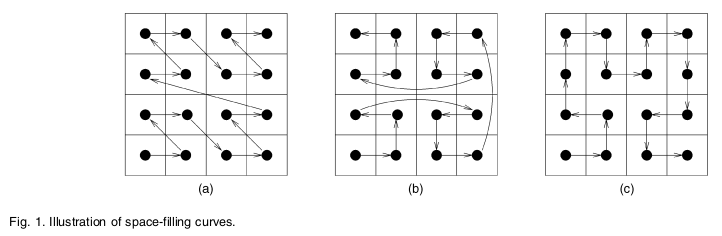
\includegraphics[width=10.cm,keepaspectratio]{Figures/space_filling_curves.png}
\end{figure}


\end{scriptsize}

\end{frame}

% -------------------------------------------------------------------------------------------------------------------


\begin{frame}
  \frametitle{Presentation of the paper}

  \centering


  \begin{figure}
  \caption{\begin{scriptsize}Analysis of the Clustering Properties of the Hilbert Space-Filling Curve. (2001) (\cite{908985})\end{scriptsize}}
  \centering
    
\includegraphics[width=10.cm,keepaspectratio]{Figures/paper_header.png}
  \end{figure}

  \begin{scriptsize}

    \begin{itemize}
      \item Analysis of the Clustering Properties of the Hilbert Space-Filling Curve. (2001)
      \item Contributions include asymptotic and exact formulas for clustering performance.
      \item Comparison against other popular space-filling curves.
    \end{itemize}
  \end{scriptsize}


\end{frame}

% -------------------------------------------------------------------------------------------------------------------

\begin{frame}
  \frametitle{Polyhedrons}

  \begin{scriptsize}
  \textbf{Queries of polyhedral shape}: \\
  Polyhedron: ``In geometry, a polyhedron is a solid in three dimensions with flat polygonal faces, straight edges and sharp corners or vertices." (Wikipedia)
  \begin{itemize}
    \item Rectilinear polyhedron: The faces are orthogonal to one axis and have right angles.
    \item Defines an interior and an exterior.
    \item In two dimensions ?
  \end{itemize}
  \end{scriptsize}

  \begin{figure}
  \caption{\begin{scriptsize}Examples of polyhedra (Wikipedia) \end{scriptsize}}
  \centering
    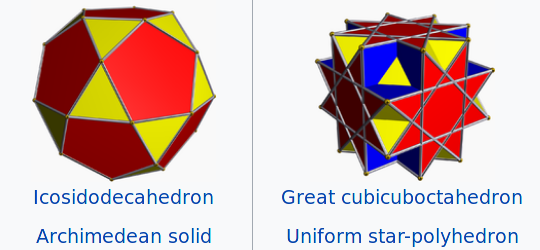
\includegraphics[width=5.cm,keepaspectratio]{Figures/polyhedra.png}
  \end{figure}

\end{frame}

%-------------------------------------------------------------------------------------------------------------------

\begin{frame}
 \frametitle{Hilbert curve}

 \begin{scriptsize}
 \begin{itemize}

   \item Defined by two parameters: d and k
   \item d: dimension of the space
   \item k: order of the curve
 \end{itemize}
 To construct the $H^d_k$ curve: take the $H^d_1$ curve and replace each point of the grid by the $H^d_{k-1}$ curve.
 \end{scriptsize}


 \begin{figure}
 \caption{\begin{scriptsize}The first three steps of the Hilbert filling curve (\cite{908985})\end{scriptsize}}
 \centering
   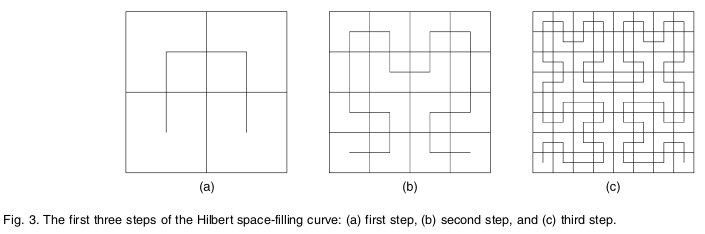
\includegraphics[width=10.cm,keepaspectratio]{Figures/hilbert_curve.png}
 \end{figure}


\end{frame}

%-------------------------------------------------
\section{Asymptotic formula of the Hilbert curve}
%-------------------------------------------------

%-------------------------------------------------------------------------------------------------------------------

\begin{frame}
 \frametitle{Clustering}

 \begin{scriptsize}
   \textbf{Definition 1}: \textit{Given a d-dimensional query, a cluster is defined
  to be a group of grid points inside the query that are consecutively connected by a mapping (or a curve).} (\cite{908985})
 \end{scriptsize}

 \begin{figure}
 \caption{\begin{scriptsize}Illustration of clustering (\cite{908985})\end{scriptsize}}
 \centering
   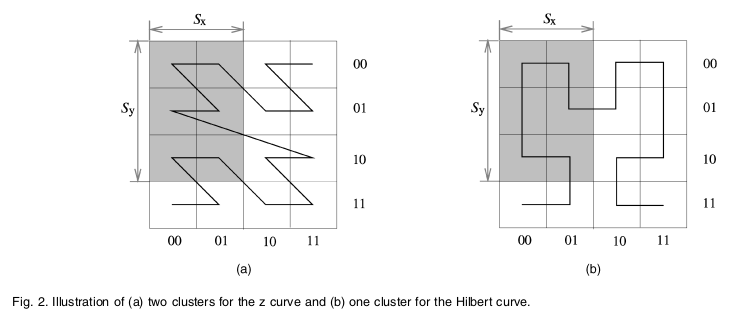
\includegraphics[width=8.cm,keepaspectratio]{Figures/clusters.png}
 \end{figure}

\begin{scriptsize}
  ``From a practical point of view, it is important to predict
and minimize the number of clusters because it determines
the number of nonconsecutive disk accesses, which, in turn,
incur additional seek time." (\cite{908985})

 \textbf{Goal}: Find a curve that reduce the number of clusters, on average, for any given query polyhedral shape.
\end{scriptsize}

\end{frame}

%-------------------------------------------------------------------------------------------------------------------

\begin{frame}
 \frametitle{Predecessors}

 \begin{scriptsize}
   Given a point $y$ in the grid:

   \begin{itemize}

     \item This point has $2d$ neighbours.
     \item One of those neighbours is a predecessor.
     \item A predecessor is the point preceding $y$ in the curve order.
     \item Probability of a neighbour $j$ parallel to dimension $i$ to be the predecessor (\cite{908985}): $$p_{ij} = p_i * \frac{1}{2} = \frac{d}{2}$$
     \item $p_i$ is the probability of the neighbour to be parallel to the $i_{th}$ dimension.

   \end{itemize}
 \end{scriptsize}
\end{frame}

%-------------------------------------------------------------------------------------------------------------------

\begin{frame}
 \frametitle{Surfaces}

 \begin{scriptsize}
   \begin{itemize}

     \item ``Border cell": Cell of the interior, close to a face.
     \item ``Potential predecessor": Cell of the exterior, close to a face.
     \item ``Surface": Aggregate number of potential predecessors.
     \item Number of entry points: $ N \approx S \frac{1}{2d} $

   \end{itemize}
 \end{scriptsize}

 \begin{figure}
 \caption{\begin{scriptsize}Illustration of faces and surfaces (\cite{908985})\end{scriptsize}}
 \centering
 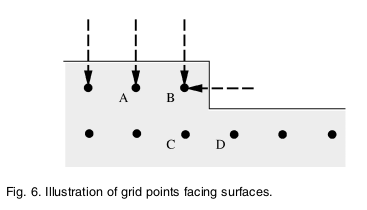
\includegraphics[width=6.cm,keepaspectratio]{Figures/faces.png}
 \end{figure}


\end{frame}

%-------------------------------------------------------------------------------------------------------------------

\begin{frame}
 \frametitle{Theorem 1 - the asymptotic formula}

 \begin{scriptsize}
  Missed one parameter: Order of the curve (resolution).

   \textbf{Theorem 1} (\cite{908985}): \textit{In a sufficiently large d-dimensional grid space
  mapped by $H^d_k$, let $S$ be the total surface area of a given
  rectilinear polyhedral query $q$. Then,}

  $$ \lim\limits_{k \to \infty} N_d = \frac{S}{2d} $$

  \textbf{Corollary} (\cite{908985}): \textit{Given a hypercube of side length $s$:}

  $$ \lim\limits_{k \to \infty} N_d = s^{d-1} $$
 \end{scriptsize}

\end{frame}


%% -------------------------------------------------------------------------------------------------------------------------

%-------------------------------------------------
\section{Experiments and comparisons}
%-------------------------------------------------

%% -------------------------------------------------------------------------------------------------------------------------

\begin{frame}
 \frametitle{Experiments}

 \begin{scriptsize}

  Experiments to test exact and asymptotic formulas \\
  Range queries of various sizes and shapes \\

   \textbf{Shapes tested:}
   \begin{itemize}

     \item 2D: square, circle, concave polygon
     \item 3D: cube, shere, concave polyhedra
     \item 4+D: hypercube, hypersphere: simpler formulas for the simulations

   \end{itemize}
   \end{scriptsize}

   \begin{figure}
   \caption{\begin{scriptsize}Shapes tested during the experiments (\cite{908985})\end{scriptsize}}
   \centering
   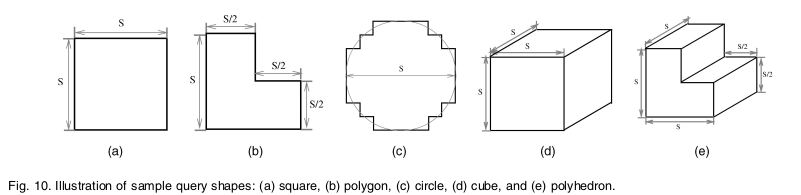
\includegraphics[width=10.cm,keepaspectratio]{Figures/shapes.png}
   \end{figure}


\end{frame}

%% -------------------------------------------------------------------------------------------------------------------------

\begin{frame}
 \frametitle{Protocol}

 \begin{scriptsize}
   \textbf{For each query:}
   \begin{itemize}

     \item Run the query on every possible points on the grid
     \item Average the numbers of clusters found

   \end{itemize}

   \textbf{Limits:}
   \begin{itemize}

     \item Not possible to do it when the dimensionality increases (Exponential):
     $$ N^d - volume\_of\_query $$
     \item Test all possibilities in 2D and 3D only + small queries
     \item Random sampling for higher dimensional space.

   \end{itemize}
 \end{scriptsize}
\end{frame}

%% -------------------------------------------------------------------------------------------------------------------------

\begin{frame}
 \frametitle{Results in 2D}

 \begin{figure}
 \caption{\begin{scriptsize}Results of the experiments in 2D (\cite{908985})\end{scriptsize}}
 \centering
 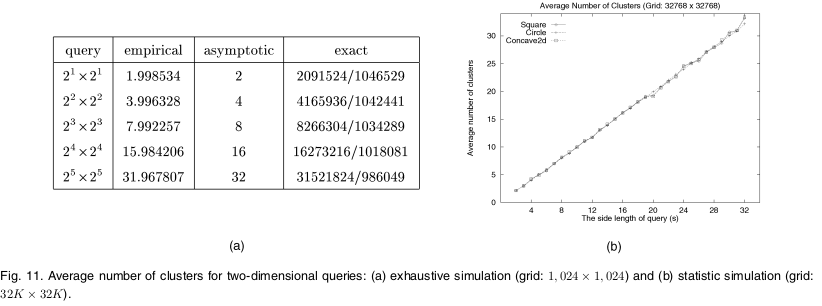
\includegraphics[width=9.cm,keepaspectratio]{Figures/res_1.png}
 \end{figure}



   \begin{scriptsize}
     \begin{itemize}

       \item (a) 1K x 1K grid space, square query: Results consistent with formulas
       \item (b) 32K x 32K grid space, 200 random queries
       \item (b) Average number of clusters in the same no matter the shape
       \item (b) The number of clusters is proportional to the query size (consistent with formula)

     \end{itemize}
   \end{scriptsize}

\end{frame}

%% -------------------------------------------------------------------------------------------------------------------------

\begin{frame}
 \frametitle{Results in 3D}

 \begin{figure}
 \caption{\begin{scriptsize}Results of the experiments in 3D and highest dimensions (\cite{908985})\end{scriptsize}}
 \centering
 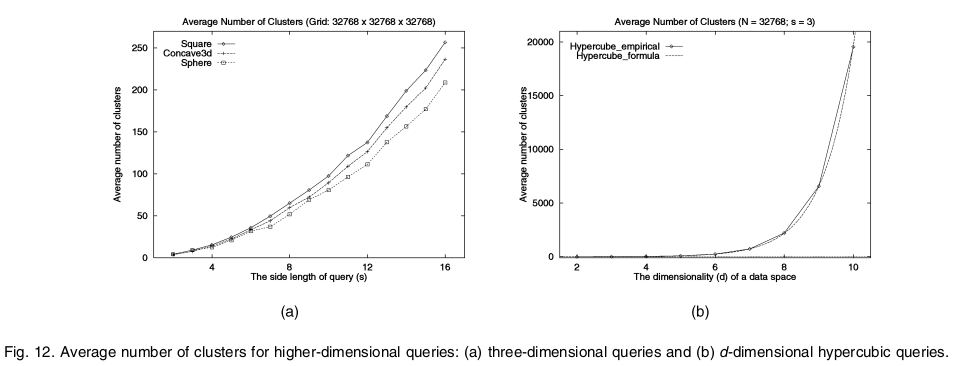
\includegraphics[width=10.cm,keepaspectratio]{Figures/res_2.png}
 \end{figure}



   \begin{scriptsize}
     \begin{itemize}

       \item (a) grid space: 32K x 32K x 32K
       \item (a) Approximate the quadratic formulas using least squares method
       \item (a) Consistent with corollary $ \lim\limits_{k \to \infty} N_d = s^{d-1} $ for the hypercube
       \item (a) Different equations for the other shapes:

     \end{itemize}

   \end{scriptsize}

\end{frame}


%% -------------------------------------------------------------------------------------------------------------------------

\begin{frame}
 \frametitle{Results in 3D}

 \begin{figure}
 \caption{\begin{scriptsize}Results of the experiments in 3D and highest dimensions (\cite{908985})\end{scriptsize}}
 \centering
 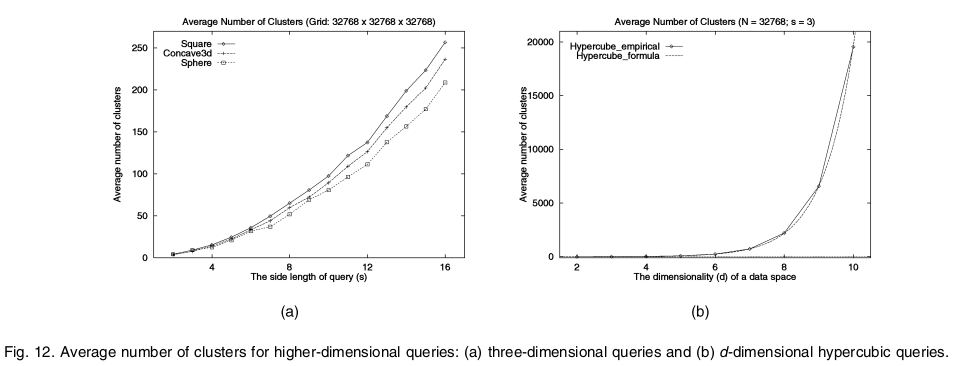
\includegraphics[width=10.cm,keepaspectratio]{Figures/res_2.png}
 \end{figure}



   \begin{scriptsize}

     \textit{[...] Unlike in the two-dimensional case,
     the surface area of a concave polyhedron or a sphere is
     smaller than that of its minimum bounding cube.} (\cite{908985})
   \end{scriptsize}

\end{frame}

%% -------------------------------------------------------------------------------------------------------------------------

\begin{frame}
 \frametitle{Results in higher dimensions}

 \begin{figure}
 \caption{\begin{scriptsize}Results of the experiments in 3D and highest dimensions (\cite{908985})\end{scriptsize}}
 \centering
 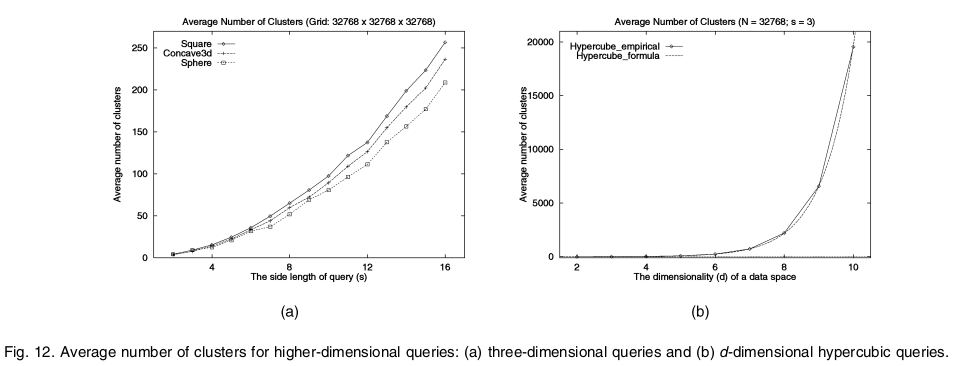
\includegraphics[width=10.cm,keepaspectratio]{Figures/res_2.png}
 \end{figure}

   \begin{scriptsize}
     \begin{itemize}
       \item (b) grid space: 32K x 32K x ... x 32K
       \item (b) queries of size 3 x 3 x ... x 3
       \item (b) Formula coincide with the asymptotic formula even in higher dimensional spaces.

     \end{itemize}
   \end{scriptsize}

\end{frame}

%% -------------------------------------------------------------------------------------------------------------------------

\begin{frame}
 \frametitle{Worst case comparisons}


 \begin{figure}
 \caption{\begin{scriptsize}Worst case comparisons between the Z, the Hilbert and the Grey-coded curves. (\cite{908985})\end{scriptsize}}
 \centering
 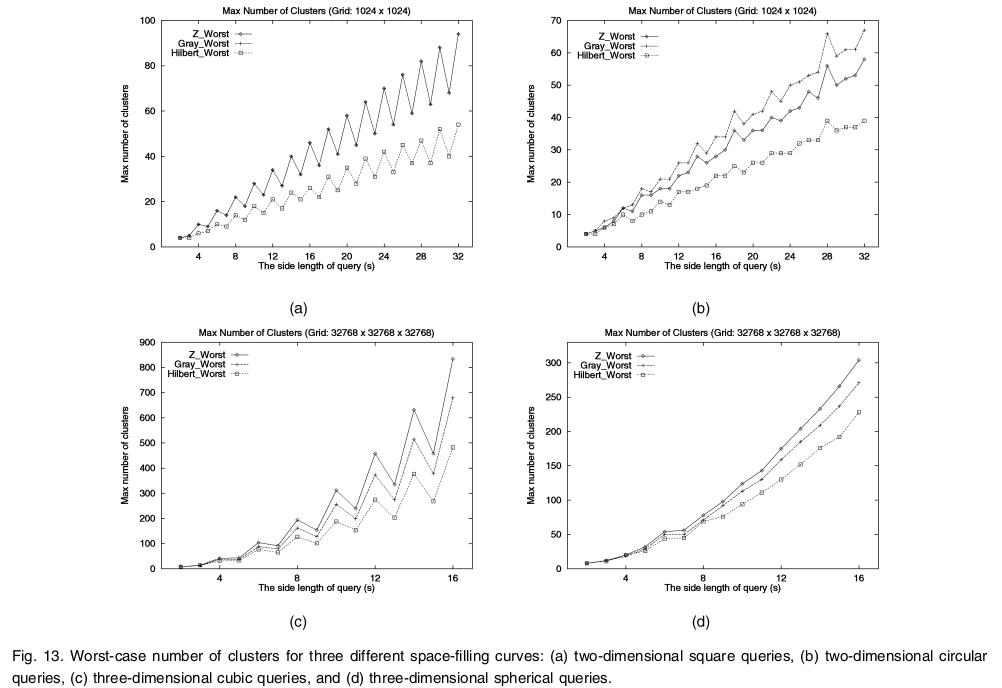
\includegraphics[width=7.cm,keepaspectratio]{Figures/worst_cases.png}
 \end{figure}


\end{frame}

%% -------------------------------------------------------------------------------------------------------------------------

\begin{frame}
 \frametitle{Average case comparisons}

 \begin{figure}
 \caption{\begin{scriptsize}Average case comparisons between the Z, the Hilbert and the Grey-coded curves. (\cite{908985})\end{scriptsize}}
 \centering
 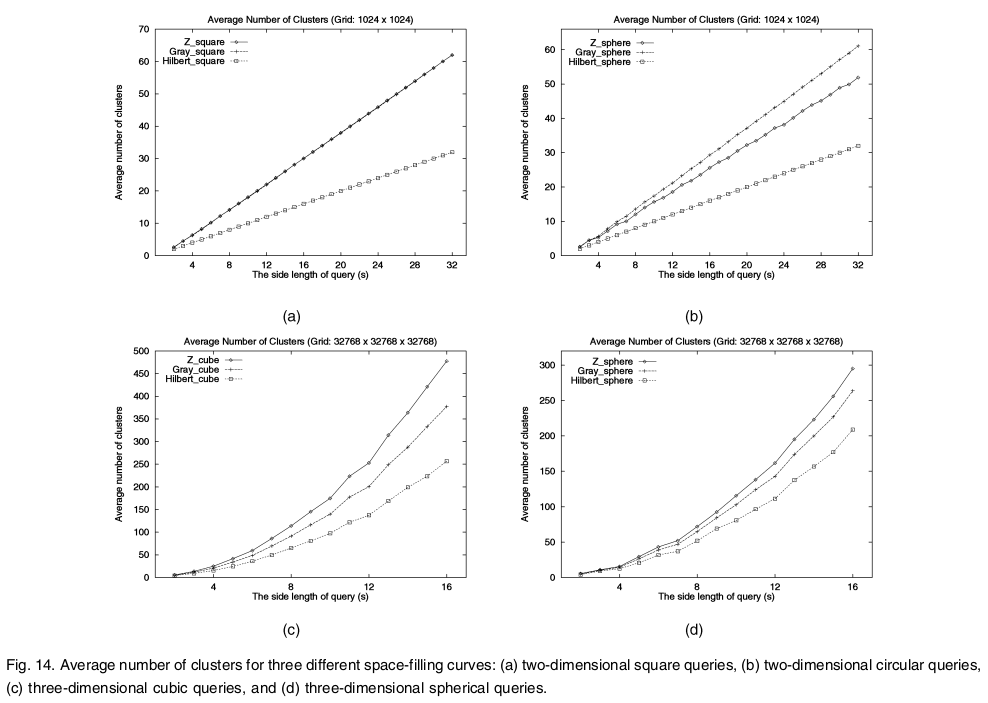
\includegraphics[width=7.cm,keepaspectratio]{Figures/average_cases.png}
 \end{figure}



\end{frame}

%% -------------------------------------------------------------------------------------------------------------------------

\begin{frame}
 \frametitle{Summary}


      ``Hilbert curve achieves
      better clustering than the z curve in a two-
      dimensional space" (\cite{908985}) \par

      In 2D: ``The average number of clusters
      for the Hilbert curve is \textbf{one-fourth} of the perimeter
      of a query rectangle, while that of the z curve is
      one-third of the perimeter plus two-thirds of the
      side length of the rectangle in the unfavored
      direction" (\cite{908985}) \par

      ``we have shown that the Hilbert curve
      outperforms both the z and Gray-coded curves in
      two-dimensional and 3-dimensional spaces. We
      conjecture that this trend will hold even in higher-dimensional spaces." (\cite{908985})


\end{frame}

%% -------------------------------------------------------------------------------------------------------------------------

%-------------------------------------------------
\section{Example of usage}
%-------------------------------------------------

%% -------------------------------------------------------------------------------------------------------------------------

\begin{frame}
  \frametitle{Data exploration of turbulence simulations using a database cluster. (2007)}

  \begin{scriptsize}
      A ``cluster of databases" (\cite{inproceedings}) to store the history of direct numerical simulations (DNS) of turbulent flows. 1024 time samples of $1024^3$ spatial points \\
      ``In fluid dynamics, turbulence or turbulent flow is any pattern of fluid motion characterized by chaotic changes in pressure and flow velocity." (Wikipedia) \\
      ``We provide real examples of how scientists use the systemto perform high-resolution turbulence research from standard desktop computing environments." \\ (\cite{inproceedings})
      Use of Morton code in a B+-tree (standard for databases indexing)
  \end{scriptsize}

  \begin{figure}
  \caption{\begin{scriptsize}Screenshot from ``Turbulent flow around a wing profile, a direct numerical simulation" (\cite{kth_mechanics}) \end{scriptsize}}
  \centering
  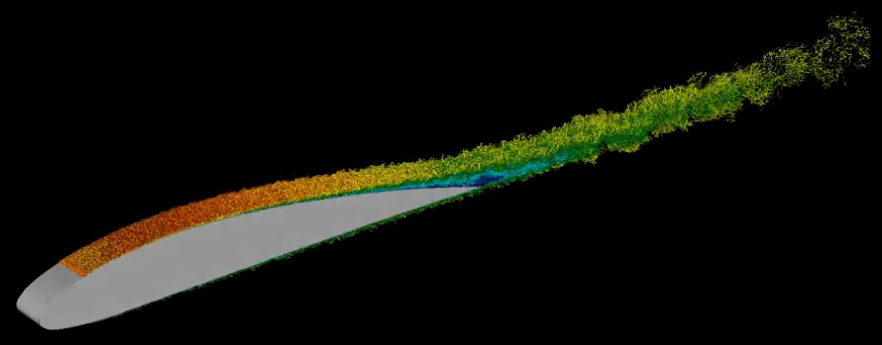
\includegraphics[width=4.cm,keepaspectratio]{Figures/high_dim.png}
  \end{figure}

\end{frame}

%% -------------------------------------------------------------------------------------------------------------------------

\begin{frame}
  \frametitle{Derivation of Morton code from the Z curve}

  \begin{figure}
  \caption{\begin{scriptsize}Illustration of how to find the Morton code. (Wikipedia) \end{scriptsize}}
  \centering
  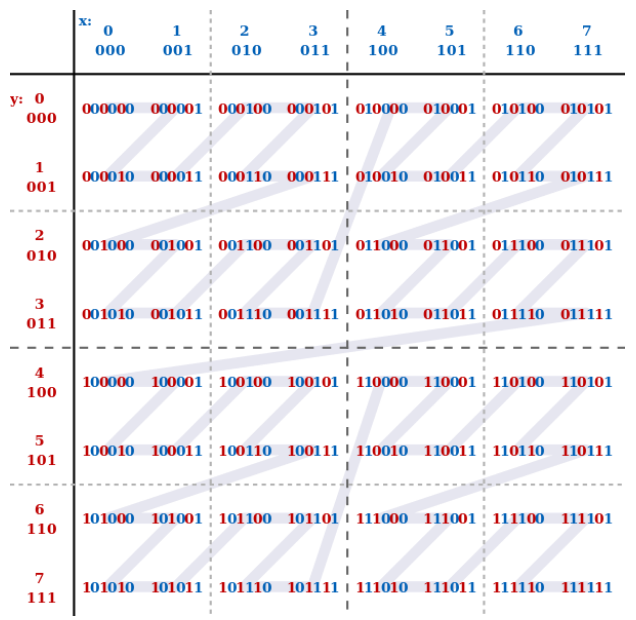
\includegraphics[width=8.cm,keepaspectratio]{Figures/morton_code.png}
  \end{figure}



\end{frame}

%% -------------------------------------------------------------------------------------------------------------------------

\begin{frame}
  \frametitle{Z-curve VS Hilbert curve}

\begin{itemize}
  \item Hilbert curve has better clustering properties than the Z-curve
  \item The Z-curve is simpler to encode/decode than the Hilbert curve.
  \item More efficient implementations of Hilbert's curve encoding/decoding now available.
  \item A new player: onion curve? (\cite{DBLP:journals/corr/abs-1801-07399})
\end{itemize}

\begin{figure}
\caption{\begin{scriptsize}Comparison of Hilbert and Onion curves (\cite{DBLP:journals/corr/abs-1801-07399}) \end{scriptsize}}
\centering
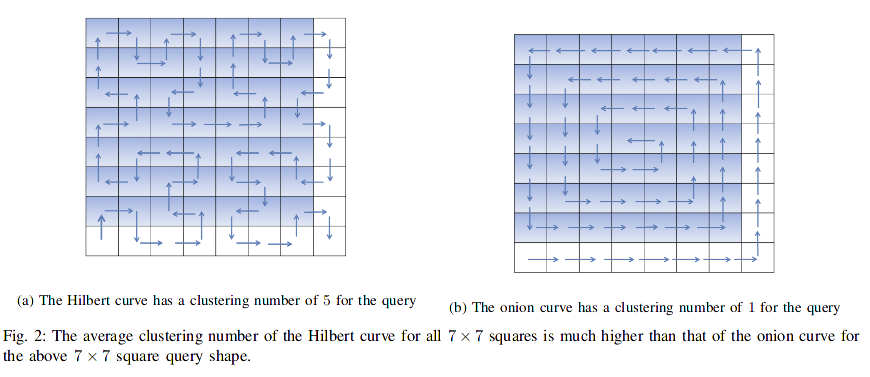
\includegraphics[width=10.cm,keepaspectratio]{Figures/onion_curve.png}
\end{figure}



\end{frame}

%% -------------------------------------------------------------------------------------------------------------------------

\begin{frame}[allowframebreaks]
\frametitle{References}

{\scriptsize

\bibliographystyle{plainnat}
\bibliography{Biblio}

}


\end{frame}

\end{document}
